This experiment is to test how static and dynamic memory allocation of Java and Rust behave. For the assessment, Element addition to ArrayList in the case of Java and Vector in the case of Rust 
is emploied here. These data stractures are resizable and we have control to set initial size. There are two parameters; initial size of ArrayList or Vector and thier final size after additions of elements. 
We are interested in the impact to memory allocation by initial allocation and expantion to runtime.

First, an ArrayList and an Vector are created with specified initial size. Then, in a loop, a element is added for each iteration until the size of the ArrayList or Vector get the specified final size. 
Each data structure has a different resizing strategy. When an ArrayList hits current limit of its size and expands the limit, it doubles the current size.  
While Vector does not have specific strategy for its resizing, the expantions of size of both ArrayList and Vector might affect the digradation of runtime performance.

To perform benchmarks, we use Java Microbenchamrk Hardness (JMH) for Java and Criterion for Rust. The benchmark time is calculated mean from several iterarions. 
We warm up before the execution. The parameters are set in combination of initial size, 10, 100, 1000, and 10000 and final size, 9, 99, 999, 9999. 
The results are shown in Figure 2-4 and 2-5. 

Discussions here are separated to two cases: when initial size is set bigger than final size and when final size is set bigger than initial size. 
For ArrayList in Java, it shows performance significant degradation when the initial size is bigger than final size. When we create ArrayList with intial size of 1000 and add 99 elements 
to the ArrayList, the the average execution time is 1125 ns. However, the average excution time when we create ArrayList with intial size of 100 and add 99 elements is 623 ns. 
This degration is caused by the cost of initializing the large array. On the other hand, Rust Vector does not have significant cost for the initialization of size compared to the cost of addition of elements. 
In the case of Vector with initial size of 1000 and add 99 elements to the Vector, the average excution is 320 ns. In the case of the initial size of 100 and 99 elements additions, 
the average excution is 279 ns. This is such small degradation compared to element addition in Vector. 

In ArrayList when the initial size is smaller than the final size, there can be degradation in performance. When its initial size and final size are set 100 and 999 respectively, 
the average execution time is 10884 ns. However when its initial size and final size are set 1000 and 999 respectively, the average execution time is 4250 ns. 
This result shows the degradation of in performance caused by the copy of existing elements into newly allocated array whose size is double of the last array.

This characteristic can be seen in the case of Vector in Rust. Vector with initial size 100 and final size 999 performs the average excution time 3514 ns, 
but one with initial size 1000 and final size 999 performs 2723 ns. When the Vector reachs its capacity, it allocates a larger buffer and copies the present elements to it.
This cost results in the degradation of the average excution time.

\begin{figure}[htb]
    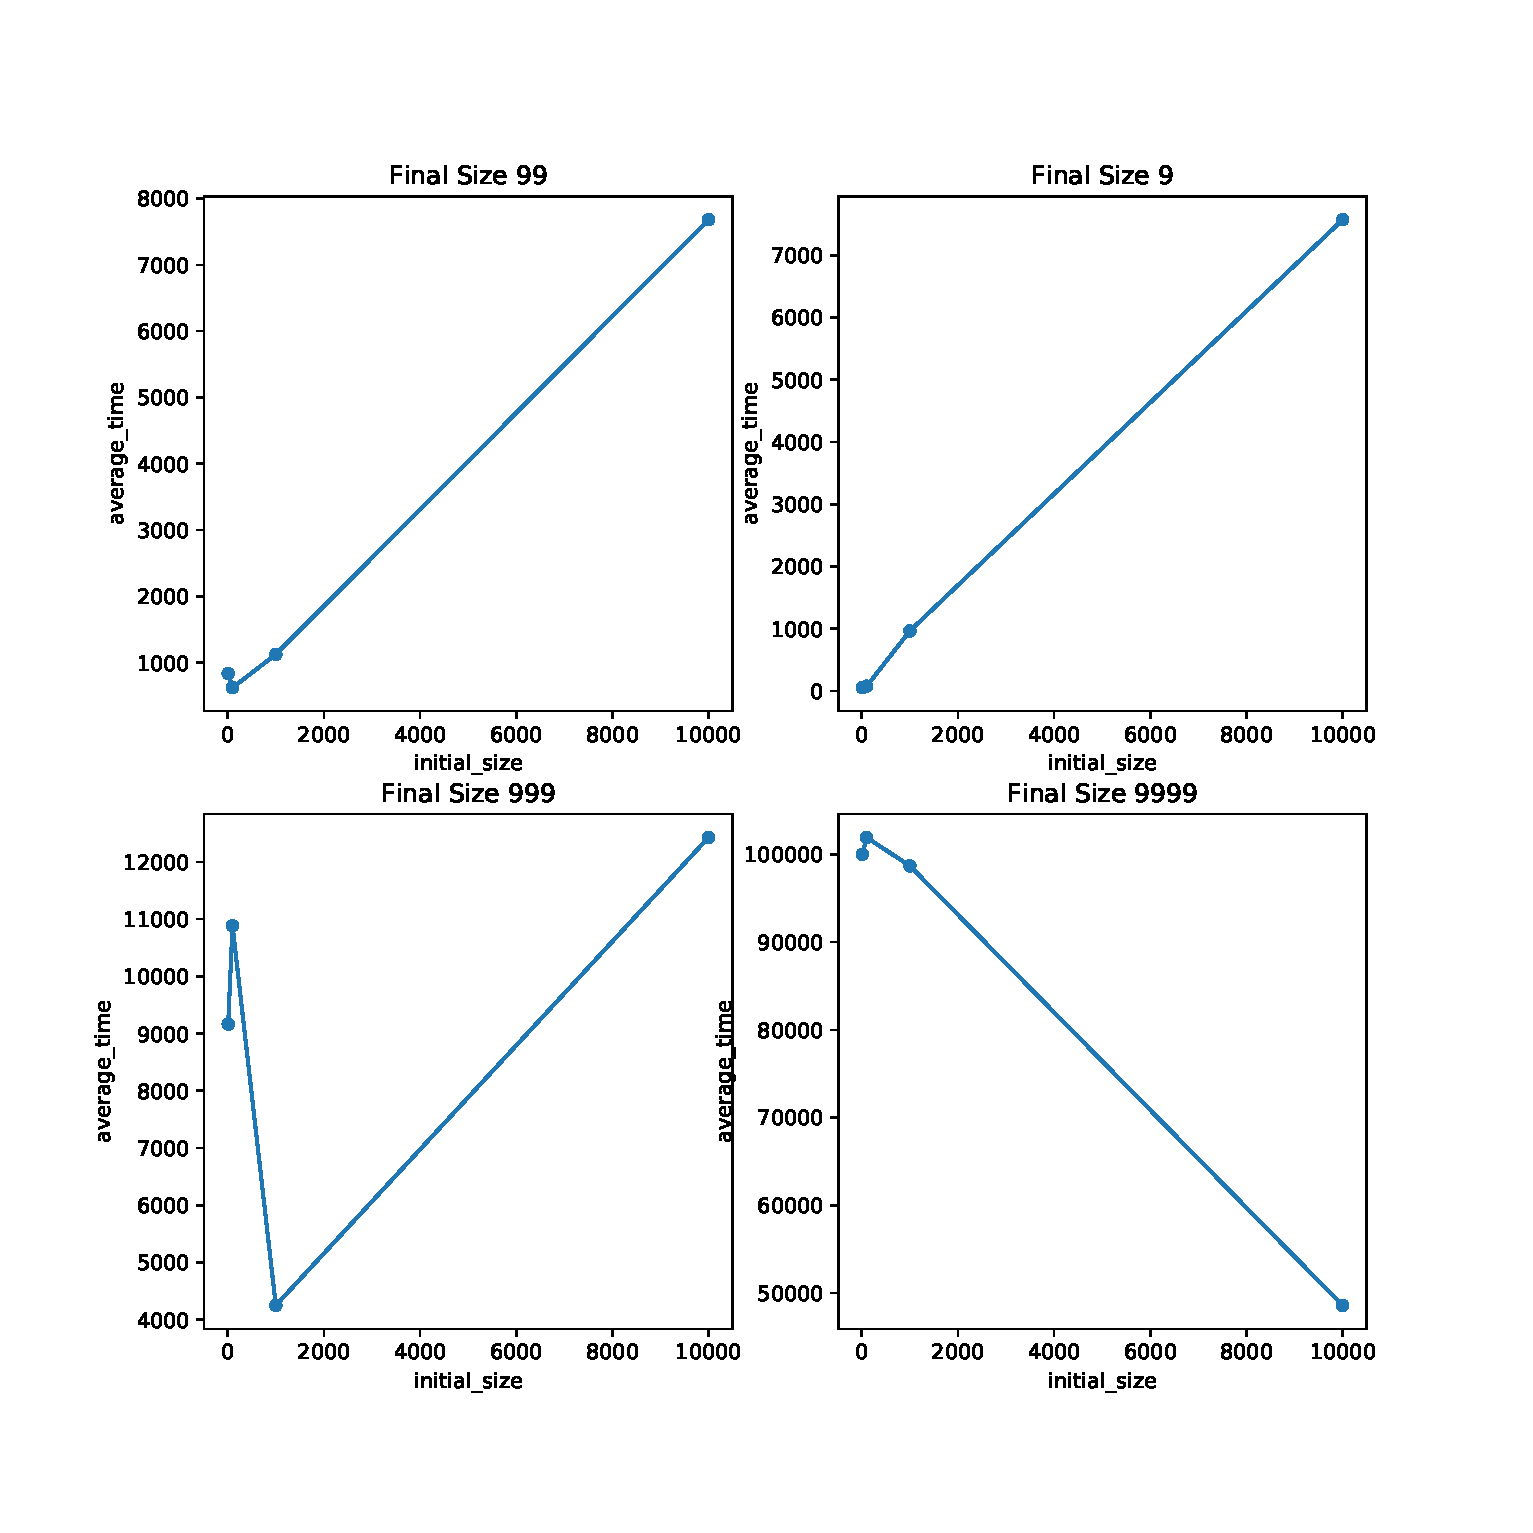
\includegraphics[width=15cm]{java_arraylist.eps}
    \caption{Memory allocation of ArrayList in Java}
    \label{fig:Sampling}
\end{figure}

\begin{figure}[htb]
    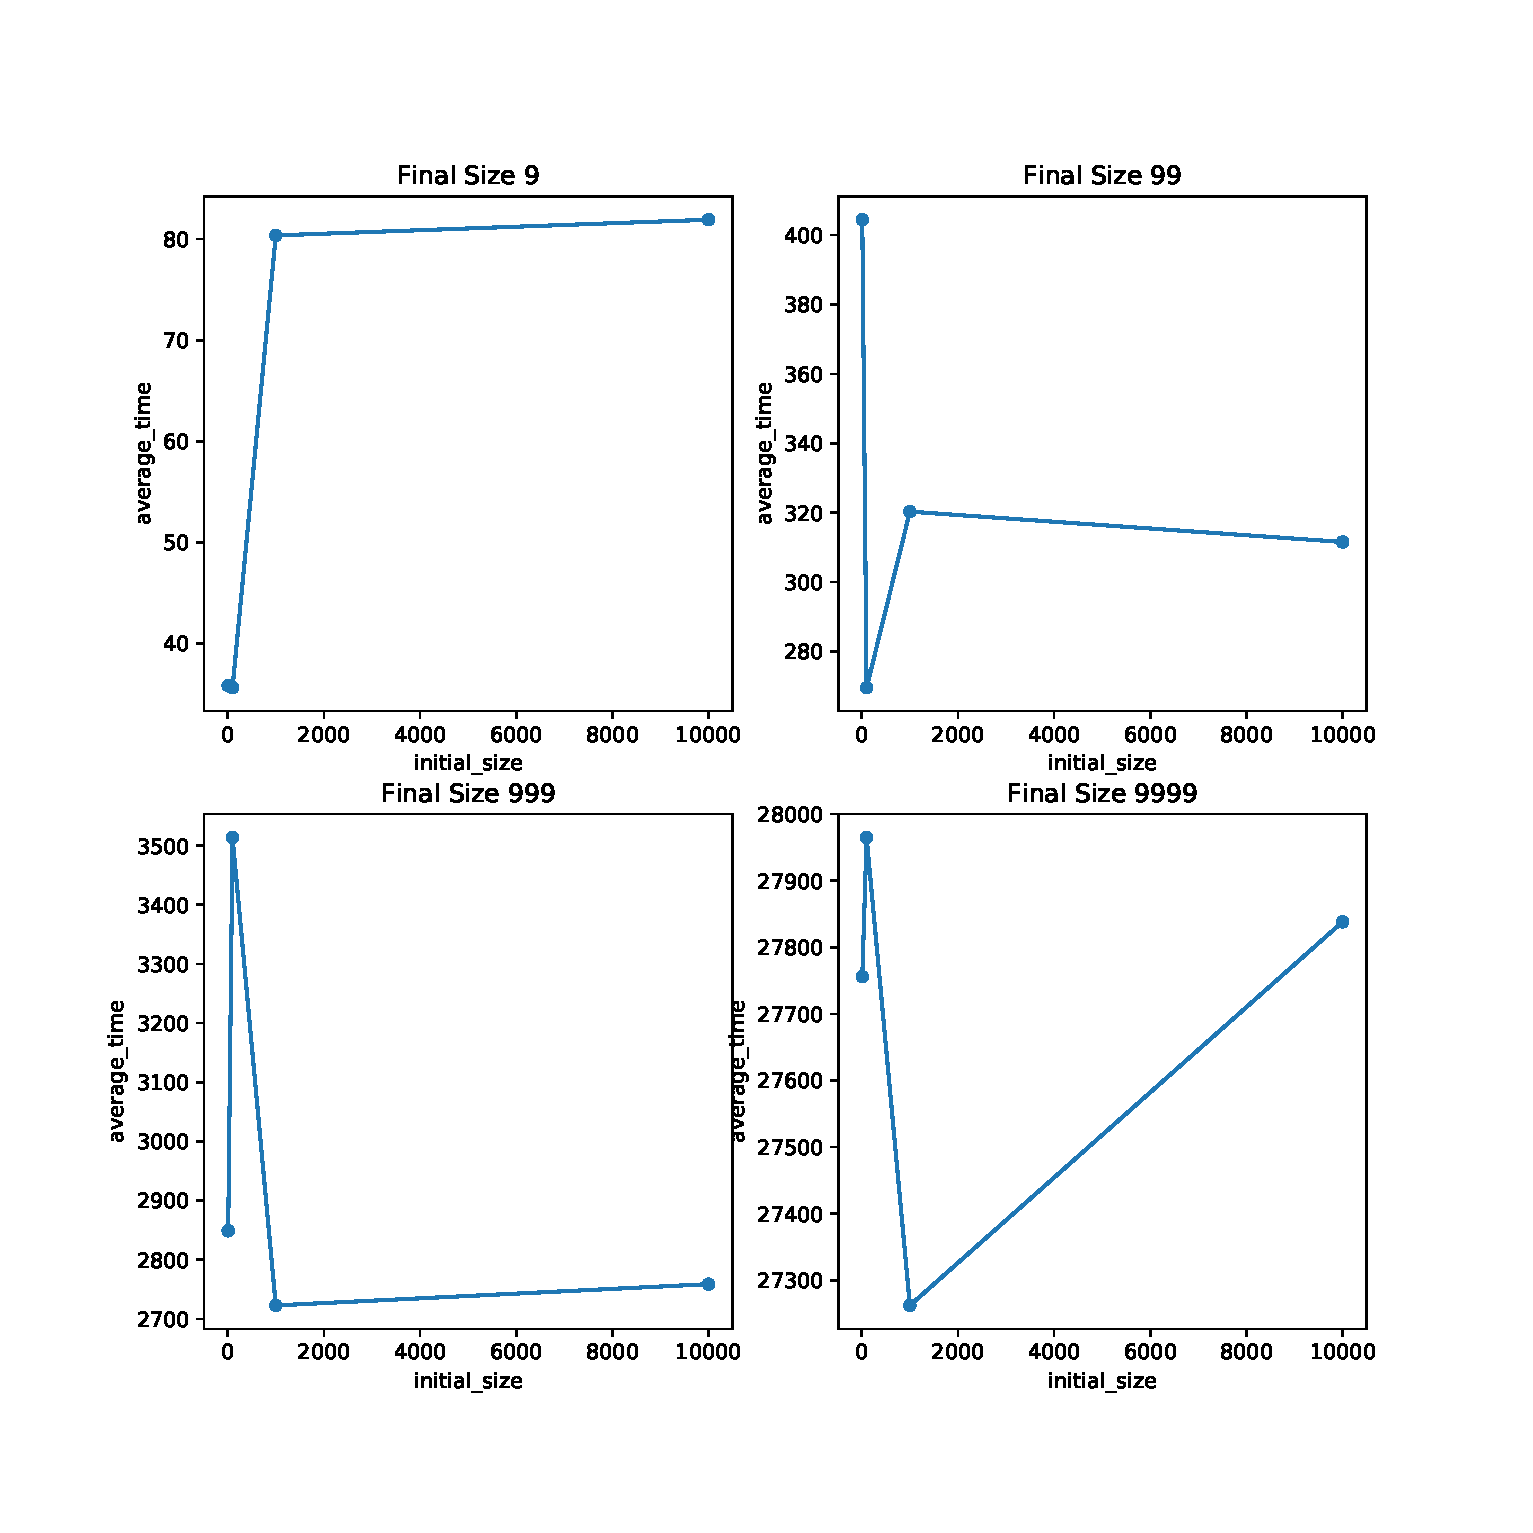
\includegraphics[width=15cm]{rust_vector.eps}
    \caption{Memory allocation of Vector in Rust}
    \label{fig:Sampling}
\end{figure}

